\documentclass[a4paper,12pt]{report}
% XeTeX/tectonic build: use fontspec + polyglossia (do not load inputenc/babel)
\usepackage[table]{xcolor}
\usepackage{graphicx}
\usepackage{titlesec}
\usepackage{fancyhdr}
\usepackage{geometry}
\usepackage{setspace}
\usepackage{tocloft}
\usepackage{hyperref}
\usepackage{polyglossia}
\usepackage{cite}
\usepackage{enumitem}
\usepackage{tabularx}
\usepackage{listings}
\usepackage{algorithm}
\usepackage[noend]{algpseudocode}

\setdefaultlanguage{thai}
\setotherlanguage{english}
\usepackage{array}

\geometry{margin=1in}
\setlength{\parindent}{2em}
\setlength{\parskip}{0pt} 
\doublespacing
\definecolor{codegreen}{rgb}{0,0.6,0}
\definecolor{codegray}{rgb}{0.5,0.5,0.5}
\definecolor{codepurple}{rgb}{0.58,0,0.82}
\definecolor{backcolour}{rgb}{0.95,0.95,0.92}

\lstdefinestyle{mystyle}{
    backgroundcolor=\color{backcolour},
    commentstyle=\color{codegreen},
    keywordstyle=\color{magenta},
    numberstyle=\tiny\color{codegray},
    stringstyle=\color{codepurple},
    basicstyle=\ttfamily\footnotesize,
    breakatwhitespace=false,
    breaklines=true,
    captionpos=b,
    keepspaces=true,
    numbers=left,
    numbersep=5pt,
    showspaces=false,
    showstringspaces=false,
    showtabs=false,
    tabsize=2
}
\lstset{style=mystyle}
% Define chapter title format
\titleformat{\chapter}[display]
  {\normalfont\Large\bfseries\centering}{บทที่ \thechapter}{1ex}{\Large}

% Define section and subsection
% Section title: Large, bold, with spacing before/after
\titleformat{\section}
  {\large\bfseries}   % Font style
  {\thesection}       % Section number
  {1em}               % Space between number and title
  {}                  % Before-code

% Subsection title: Normal size
\titleformat{\subsection}
  {\normalsize\bfseries}
  {\thesubsection}
  {1em}
  {}

% Header and footer
\pagestyle{fancy}
\fancyhf{}
\fancyfoot[C]{\thepage}

% thai language support
\usepackage{fontspec}
\setmainfont[
  Path = ./fonts/,                  % Path to the fonts folder
  UprightFont = THSarabun,           % Regular (upright) font
  BoldFont = THSarabun-Bold,         % Bold font
  ItalicFont = THSarabun-Italic,     % Italic font
  BoldItalicFont = THSarabun-BoldItalic, % Bold-Italic font
  Scale = 1.5
]{THSarabun}
% Explicitly bind Thai and Latin/English fonts for polyglossia
\newfontfamily\thaifont[
  Path = ./fonts/,
  UprightFont = THSarabun,
  BoldFont = THSarabun-Bold,
  ItalicFont = THSarabun-Italic,
  BoldItalicFont = THSarabun-BoldItalic,
  Script=Thai
]{THSarabun}
\newfontfamily\thaifonttt[
  Path = ./fonts/,
  UprightFont = THSarabun,
  BoldFont = THSarabun-Bold,
  ItalicFont = THSarabun-Italic,
  BoldItalicFont = THSarabun-BoldItalic,
  Script=Thai
]{THSarabun}

\newfontfamily\englishfont[
  Path = ./fonts/,
  UprightFont = THSarabun,
  BoldFont = THSarabun-Bold,
  ItalicFont = THSarabun-Italic,
  BoldItalicFont = THSarabun-BoldItalic
]{THSarabun}
\newfontfamily\latinfont[
  Path = ./fonts/,
  UprightFont = THSarabun,
  BoldFont = THSarabun-Bold,
  ItalicFont = THSarabun-Italic,
  BoldItalicFont = THSarabun-BoldItalic
]{THSarabun}
\XeTeXlinebreaklocale "th"
\XeTeXlinebreakskip = 0pt plus 1pt

% For dotted underline
\usepackage{tikz}
\newcommand{\uloosdot}[1]{%
    \tikz[baseline=(todotted.base)]{
        \node[inner sep=1pt,outer sep=0pt] (todotted) {#1};
        \draw[loosely dotted] (todotted.south west) -- (todotted.south east);
    }%
}%

% Thai page number
% Thai letters as page numbers
\newcommand{\thaipagenum}{
  \ifcase\value{page}
    \or ก%
    \or ข%
    \or ค%
    \or ง%
    \or จ%
    \or ฉ%
    \or ช%
    \or ซ%
    \or ฌ%
    \else หน้า~\thepage % fallback
  \fi
}

\usepackage{tocbibind}
\usepackage{indentfirst}
\usepackage{algorithmicx}
\emergencystretch=3em

\begin{document}

% Cover Page
\begin{titlepage}
    \thispagestyle{empty}
    \vspace*{\fill}  % Push content to vertical center
    \begin{center}
        \textbf{\Large รายงานปฏิบัติงานสหกิจศึกษา}\\[0.5cm]
        \textbf{\Large Japan Advanced Instituted of Science and Technology}\\[3cm]
        \Large \textbf{KGs-Augmented Test Suite Generation via Re-construct Accident Report}\\
        \textbf{\Large นาย ชัยภัทร ใจน่าน}\\
        \textbf{\Large 650510606}\\[3cm]
        \textbf{\large สหกิจศึกษานี้เป็นส่วนหนึ่งของการศึกษาหลักสูตรปริญญาวิทยาศาสตรบัณฑิต} \\
        \textbf{\large สาขาวิชาวิทยาการคอมพิวเตอร์}\\
        \textbf{\large คณะวิทยาศาสตร์ มหาวิทยาลัยเชียงใหม่}\\
        \textbf{\large ปีการศึกษา 2565}
    \end{center}
    \vspace*{\fill} 
\end{titlepage}

% Approval Page
\newpage
\clearpage
\thispagestyle{empty}
\setcounter{page}{0}

\begin{center}
    \large \textbf{รายงานปฏิบัติงานสหกิจศึกษา}\\[0.5cm]
    \textbf{KGs-Augmented Test Suite Generation via Re-construct Accident Report}\\[3cm]
    \normalsize นาย ชัยภัทร ใจน่าน\\
    650510606\\[3cm]
    สหกิจศึกษานี้เป็นส่วนหนึ่งของการศึกษาหลักสูตรปริญญาวิทยาศาสตรบัณฑิต \\
    สาขาวิชาวิทยาการคอมพิวเตอร์\\
    คณะวิทยาศาสตร์ มหาวิทยาลัยเชียงใหม่\\
    ปีการศึกษา 2567\\[2cm]
    \normalsize คณะกรรมการสอบสหกิจศึกษา\\[1cm]
    \begin{tabular}{c l}
        \uloosdot{\phantom{xxxxxxxxxxxxxxxxxxxxxxxxxxx}} & ประธานกรรมการ \\
        ( ผศ.ดร.อารีรัตน์ ตรงรัศมีทอง ) & \\
         & \\
        \uloosdot{\phantom{xxxxxxxxxxxxxxxxxxxxxxxxxxx}} & กรรมการ \\
        ( ผศ.ดร.เสมอแข สมหอม ) & \\
    \end{tabular} \\[1cm]
    วันที่ \uloosdot{\phantom{xxx}} เดือน \uloosdot{\phantom{xxxxxxxxx}} พ.ศ. \uloosdot{\phantom{xxxxxx}}
\end{center}

\newpage
\clearpage
\thispagestyle{empty}
\setcounter{page}{0}
หนังสือยิมยอมให้ข้อมูลเพื่อการศึกษา

\newpage
\clearpage
\renewcommand{\thepage}{\thaipagenum}
\setcounter{page}{1}

% Acknowledgements
\chapter*{กิตติกรรมประกาศ}
\addcontentsline{toc}{chapter}{กิตติกรรมประกาศ}
\paragraph{} ข้าพเจ้าขอขอบพระคุณอาจารย์ที่ปรึกษาสหกิจศึกษา ผศ.ดร.อารีรัตน์ ตรงรัศมีทอง ที่ได้ให้คำแนะนำ
และช่วยแก้ไขปัญหาต่าง ๆ ตลอดระยะเวลาการทำงาน
\begin{flushright}
    นาย ชัยภัทร ใจน่าน\\
    650510606
\end{flushright}
% (insert acknowledgements here)

% Abstract
{
\cleardoublepage% Move to first page of new chapter
\let\clearpage\relax% Don't allow page break
\noindent
\begin{tabular}{l p{10cm}}
    \textbf{หัวข้อสหกิจศึกษา} & การสร้างชุดทดสอบเสริมด้วย Knowledge Graphs ผ่านการสร้างรายงานอุบัติเหตุซ้ำ \vspace{0.2cm} \\
    \textbf{สถานประกอบการ} & Japan Advanced Instituted of Science and Technology \vspace{0.2cm}\\
    \textbf{ผู้ดำเนินการศึกษา} & ชัยภัทร ใจน่าน (Chaipat Jainan) \vspace{0.2cm}\\
    \textbf{หลักสูตร} & วิทยาศาสตรบัณฑิต สาขาวิชาวิทยาการคอมพิวเตอร์ \vspace{0.2cm}\\
    \textbf{อาจารย์ที่ปรึกษาสหกิจ} & ผศ.ดร.อารีรัตน์ ตรงรัศมีทอง \vspace{0.2cm}\\
\end{tabular}

\chapter*{บทคัดย่อ}
\addcontentsline{toc}{chapter}{บทคัดย่อ}

\paragraph{}
งานวิจัยนี้มีวัตถุประสงค์เพื่อแก้ไขปัญหาด้านความน่าเชื่อถือและประสิทธิภาพในการสร้างชุดทดสอบสำหรับระบบขับขี่อัตโนมัติ (ADS) จากรายงานอุบัติเหตุจริง แม้ว่าโมเดลภาษาขนาดใหญ่ (LLM) จะมีศักยภาพในการสร้างสถานการณ์จำลอง แต่การใช้งานโดยตรงยังขาดกลไกในการมุ่งเน้นไปยังกรณีขอบเขต (Edge-Case) ที่ชัดเจน ซึ่งส่งผลให้เกิดการสร้างสถานการณ์จำลองที่ไม่จำเป็นจำนวนมาก งานวิจัยจึงนำเสนอกรอบการทำงานสำหรับการสร้างชุดทดสอบที่น่าเชื่อถือและมุ่งเน้นเป้าหมาย โดยใช้ Schema-guided LLM ในการสกัดข้อมูลอุบัติเหตุที่มีโครงสร้าง ก่อนนำไปสร้างเป็น Knowledge Graph (KG) เพื่อใช้เป็นโครงสร้างเชิงความหมายที่ช่วยในการอนุมานข้อมูลและความต่อเนื่องเชิงเหตุผล หัวใจสำคัญของกรอบการทำงานนี้คือการบูรณาการ Operational Design Domain (ODD) ที่กำหนดโดย Japan Automobile Manufacturers Association (JAMA) เข้าไปใน KG เพื่อใช้เป็นหลักเกณฑ์ในการกรองและควบคุมการสร้าง Scenario ให้มุ่งเน้นการค้นพบ Edge-Case ใหม่ ๆ ได้อย่างรวดเร็วและมีประสิทธิภาพ ผลลัพธ์ที่ได้คือก้าวสำคัญในการพัฒนาวิธีการสร้างชุดทดสอบที่มีความแม่นยำสูง ซึ่งช่วยลดจำนวนครั้งในการสร้างเหตุการณ์จำลองซ้ำ และสนับสนุนการรับรองความปลอดภัยของระบบ ADS ได้อย่างเป็นรูปธรรม
}


\newpage
{
\cleardoublepage% Move to first page of new chapter
\let\clearpage\relax% Don't allow page break
\noindent
\begin{tabular}{l l c}
    \textbf{Title} & KGs-Augmented Test Suite Generation via Re-construct Accident Report & \vspace{0.2cm}\\
    \textbf{Company} & Japan Advanced Instituted of Science and Technology & \vspace{0.2cm}\\
    \textbf{Name} & Chaipat Jainan & \vspace{0.2cm}\\
    \textbf{ID} & 650510606 & \vspace{0.2cm}\\
    \textbf{Degree} & Bachelor of Science in Computer Science & \vspace{0.2cm}\\
    \textbf{Advisor} & Asst. Prof. Areerat Trongratsameethong & \vspace{0.2cm}\\
\end{tabular}

\chapter*{Abstract}
\addcontentsline{toc}{chapter}{Abstract}

\paragraph{}
Ensuring the safety of Autonomous Driving Systems (ADS) necessitates rigorous testing using simulated scenarios derived from real-world accident reports. While Large Language Models (LLMs) offer a promising approach for generating these scenarios, their direct application in discovering elusive edge-cases is often inefficient and unreliable. This inefficiency stems primarily from the inconsistent nature of the source reports and the LLMs' tendency to generate numerous irrelevant scenarios, leading to an unnecessarily high number of reconstruction efforts before a novel test case is found.

To address this challenge, this study proposes a novel KGs-Augmented Testsuite Generator Framework designed to create reliable and goal-oriented test suites. The framework employs a schema-guided LL to accurately extract structured accident data from unstructured reports. This data is then modeled as a Knowledge Graph (KG), which serves as a semantic backbone, enabling robust inference of missing information and maintaining the causal continuity between events. Crucially, the framework integrates the Operational Design Domain (ODD), utilizing constraints defined by JAMA, directly into the KG structure.

The integration of ODD acts as a powerful filter and guideline, controlling the scenario generation process to focus exclusively on test cases that violate or push the boundaries of the defined operational limits. This targeted approach is the key to the framework's effectiveness, which aims to significantly reduce the number of reconstructed scenarios required to discover a new, challenging edge-case. The resulting structured scenarios are highly reliable and compliant with industry standards (e.g., ASAM OpenSCENARIO), marking a substantial improvement in the efficiency and quality of ADS safety evaluation.
}
\newpage
% Table of Contents
\renewcommand{\contentsname}{สารบัญ}
\renewcommand{\listfigurename}{สารบัญรูป}
\renewcommand{\listtablename}{สารบัญตาราง}
\tableofcontents
\newpage
\listoffigures
\newpage
\listoftables

% Revert back to arabic page number
\cleardoublepage
\renewcommand{\thepage}{\arabic{page}}
\setcounter{page}{1}
\pagenumbering{arabic}

% Chapters
\renewcommand{\figurename}{รูปที่}
\renewcommand{\tablename}{ตารางที่}
\renewcommand\bibname{บรรณานุกรม}
\chapter{บทนำ}\label{ch:introduction}

\paragraph{}{\sloppy การปฏิบัติงานสหกิจครั้งนี้ผู้จัดทำได้ปฏิบัติงานที่ Japan Advanced Instituted of Science and Technology (JAIST) ซึ่งได้รับมอบหมายงานเกี่ยวกับการออกแบบเฟรมเวิร์ค (Framework) สำหรับการสร้างชุดทดสอบของระบบขับเคลื่อนอัตโนมัติของ รถยนต์โดยนำเอาความรู้เรื่องโครงสร้างกราฟความรู้ (Knowledge Graph) มาประยุกต์ใช้ \par}

\section{ข้อมูลสถานประกอบการ}\label{sec:company-info}

\subsection{ชื่อองค์กร}\label{subsec:company-name}
\paragraph{}Japan Advanced Instituted of Science and Technology (JAIST)

\subsection{ระยะเวลาการปฏิบัติงาน}\label{subsec:duration}
\paragraph{}ตั้งแต่วันที่ 14 เมษายน พ.ศ.2568 จนถึงวันที่ 30 กันยายน พ.ศ.2568

\subsection{ลักษณะขององค์กร}\label{subsec:company-type}
\paragraph{}Japan Advanced Institute of Science and Technology เป็นมหาวิทยาลัยในประเทศญี่ปุ่นที่จัดการศึกษาในระดับบัณฑิตศึกษา ซึ่งแบ่งสาขาวิชาตามหัวข้อศึกษาหลักที่มีอยู่ 3 หัวข้อดังนี้

\begin{enumerate}[label=\arabic*.)]
    \item Knowledge Science: สาขาวิชาที่บูรณาการความรู้เกี่ยวกับวิธีการออกแบบ
การจัดการธุรกิจ วิทยาศาสตร์ระบบ (System Science)
และความรู้อื่นๆ ที่เกี่ยวข้องกับปัญหาของมนุษย์ องค์กร
หรือสังคมเพื่อเสนอวิธีแก้ปัญหาเหล่านั้นและพิจารณาว่าจะทำให้วิธีแก้ปัญหาเป็นรูปธรรมได้อย่างไร
    \item Information Science: เป็นสาขาวิชาที่มุ่งเน้นการแก้ไขปัญหาสำหรับมนุษย์และสังคม
การสร้างทฤษฎีพื้นฐานใหม่ๆ ที่เป็นนวัตกรรมและการประยุกต์การประมวลผลข้อมูลเข้ากับการสื่อสารเพื่อรองรับสังคมยุคใหม่ที่ขับเคลื่อนด้วยข้อมูล
    \item Material Science: เป็นสาขาวิชาการที่มุ่งผลิตวัสดุใหม่และนวัตกรรมโดยมุ่งแก้ปัญหาให้กับมนุษยชาติและสังคม
และบุกเบิกสาขาที่ยังไม่มีการสำรวจบนพื้นฐานของฟิสิกส์ เคมี ชีววิทยา
และวิทยาศาสตร์และเทคโนโลยีที่เกี่ยวข้อง
\end{enumerate}

\section{ตำแหน่งและลักษณะงานที่ได้รับมอบหมาย}\label{sec:job-details}

\subsection{ตำแหน่งงานที่ปฏิบัติ}\label{subsec:job-position}
\paragraph{}Research Intern
\subsection{งานที่ได้รับมอบหมาย}\label{subsec:assigned-tasks}

\paragraph{}ออกแบบเฟรมเวิร์ค
(Framework)
สำหรับการสร้างชุดทดสอบประสิทธิภาพการทำงานของระบบ
ขับเคลื่อนอัตโนมัติของรถยนต์
เพื่อให้ผู้พัฒนาระบบขับเคลื่อนอัตโนมัติสามารถสร้างชุดทดสอบของตนเอง เพื่อนำไป
ปรับปรุง ปรับใช้ และทดสอบระบบของตนเอง

\section{หลักการและเหตุผล}\label{sec:introduction}


\paragraph{}งานวิจัย KGs-Augmented Test Suite Generation via Re-construct Accident Report มุ่งเน้นการแก้ปัญหาหลักในการทดสอบระบบขับขี่อัตโนมัติ (ADS) นั่นคือ ต้องสร้างเคสจำลองจำนวนมากจนกว่าจะพบ Edge-Case ใหม่ ปัจจุบัน การใช้ Large Language Models (LLMs) เพื่อสร้างสถานการณ์จำลองจากรายงานอุบัติเหตุจริงยังคงมีข้อจำกัดด้านความน่าเชื่อถือ เนื่องจากขาดโครงสร้างข้อมูลที่ชัดเจนและเป้าหมายการทดสอบที่สอดคล้องกับขอบเขตการทำงานของระบบ (ADS) ที่กำหนดไว้ ซึ่งส่งผลให้มีการสร้าง Scenario ที่ไม่จำเป็นจำนวนมาก จนกว่าจะพบเคสที่ท้าทายระบบจริง งานวิจัยนี้จึงถือกำเนิดขึ้นเพื่อพัฒนาแนวทางที่เป็นระบบ โดยมีวัตถุประสงค์หลักเพื่อ ลดจำนวนเหตุการณ์ที่ต้องสร้างใหม่ ให้ได้มากที่สุด และเพิ่มอัตราส่วนการค้นพบ Edge-Case

กรอบการทำงานที่นำเสนอประกอบด้วยการทำงานร่วมกันของเทคโนโลยีหลักสามส่วนเพื่อเพิ่มประสิทธิภาพดังกล่าว: 1) Schema-guided LLM ถูกใช้เพื่อสกัดข้อมูลอุบัติเหตุจากรายงานข้อความให้อยู่ในรูปแบบที่มีโครงสร้าง 2) Knowledge Graph (KG) ถูกใช้เป็นโครงสร้างเชิงความหมาย (Semantic Backbone) ในการจัดเก็บข้อมูล ทำให้สามารถอนุมานข้อมูลที่ขาดหายไปและรักษาความต่อเนื่องเชิงเหตุผลของเหตุการณ์ได้อย่างแม่นยำ และที่สำคัญที่สุดคือ 3) การผสานรวม Operational Design Domain (ODD) ที่กำหนดโดย JAMA เข้าไปใน KG โดย ODD นี้ทำหน้าที่เป็นไกด์ไลน์และตัวกรอง เพื่อจำกัดการสร้าง Scenario ให้มุ่งเน้นเฉพาะสถานการณ์ที่อยู่ในขอบเขตการทำงานของ ADS เท่านั้น ซึ่งถือเป็นการควบคุมทิศทางของการสร้างชุดทดสอบให้ มุ่งเป้าหมายสู่ Edge-Case ที่เกี่ยวข้อง โดยตรง

ผลลัพธ์ที่คาดว่าจะได้รับจากโครงการนี้คือ กรอบการทำงานที่เชื่อถือได้และมีประสิทธิภาพสูง ในการสร้างชุดทดสอบสำหรับ ADS ประโยชน์ที่สำคัญที่สุดคือการช่วยให้นักวิจัยและผู้พัฒนาสามารถ เพิ่มความเร็วในการค้นพบสถานการณ์ทดสอบที่สำคัญ ด้วยทรัพยากรที่น้อยลง ชุดทดสอบที่สร้างขึ้นจะมีความน่าเชื่อถือสูง เนื่องจากมีโครงสร้างและมีความสอดคล้องกับเงื่อนไข ODD ทำให้การประเมินความปลอดภัยของระบบ ADS มีความเข้มงวดและมีคุณภาพมากขึ้น ซึ่งเป็นการวางรากฐานสำคัญสำหรับการรับรองความปลอดภัยของยานยนต์อัตโนมัติในอนาคต

\section{วัตถุประสงค์}\label{sec:objectives}

\begin{enumerate}[label=\arabic*.)]
    \item พัฒนากรอบการสร้างชุดทดสอบที่มีความน่าเชื่อถือที่เรียกว่า KGs-Augmented Testsuite Generator ซึ่งสามารถสกัดข้อมูลอุบัติเหตุแบบมีโครงสร้างจากรายงานที่เป็นข้อความโดยใช้ Schema-guided LLM และสร้างเป็น Knowledge Graph (KG) เพื่อใช้เป็นรากฐานเชิงความหมายของข้อมูลอุบัติเหตุ
    \item เพิ่มประสิทธิภาพการค้นพบ Edge-Case โดยการบูรณาการ Operational Design Domain (ODD) ที่กำหนดโดย JAMA เข้ากับ Knowledge Graph เพื่อใช้เป็นตัวกรองและหลักเกณฑ์ในการควบคุมการสร้าง Scenario ให้มุ่งเน้นเฉพาะสถานการณ์ที่ท้าทายระบบ (Edge-Case) ซึ่งเป็นไปตามวัตถุประสงค์หลักของงานวิจัยคือ การลดจำนวนเหตุการณ์ที่จำเป็นต้องสร้างใหม่จนกว่าจะพบเเคสใหม่
    \item สร้างชุดทดสอบอุบัติเหตุที่มีโครงสร้างที่สมบูรณ์และถูกต้องตามหลักเหตุผล ซึ่งสามารถส่งออกในรูปแบบมาตรฐาน เช่น ASAM OpenSCENARIO เพื่อนำไปใช้งานในการจำลองการทดสอบ ระบบขับขี่อัตโนมัติได้อย่างมีประสิทธิภาพและตรงเป้าหมาย
\end{enumerate}

\section{ประโยชน์ที่คาดว่าจะได้รับ}\label{sec:expected-benefits}

\begin{enumerate}[label=\arabic*.)]
    \item การเพิ่มประสิทธิภาพในการค้นพบ Edge-Case: กรอบการทำงานนี้จะช่วยให้นักวิจัยและผู้พัฒนาระบบสามารถลดจำนวนเหตุการณ์จำลองที่ไม่จำเป็นลงได้อย่างมาก เนื่องจากมีการใช้ ODD เป็นไกด์ไลน์ในการกรองและควบคุมการสร้าง Scenario ให้มุ่งเน้นเฉพาะสถานการณ์ที่อยู่ในขอบเขตการทำงานของ ADS และท้าทายระบบจริง ๆ เท่านั้น ซึ่งนำไปสู่การประหยัดเวลาและทรัพยากรในการทดสอบ
    \item การยกระดับความน่าเชื่อถือของชุดทดสอบ: ชุดทดสอบที่สร้างขึ้นจาก Knowledge Graph มีความถูกต้องเชิงโครงสร้างและรักษาความต่อเนื่องเชิงเหตุผล (Causal Continuity) ของเหตุการณ์อุบัติเหตุ ทำให้ผลการประเมินระบบขับขี่อัตโนมัติมีความน่าเชื่อถือและสอดคล้องกับความเป็นจริงมากขึ้น
    \item การเป็นรากฐานสำหรับงานวิจัยต่อยอด: Knowledge Graph ที่สร้างขึ้นจากข้อมูลอุบัติเหตุจริงและผสานรวมกับเงื่อนไข ODD สามารถทำหน้าที่เป็นแหล่งข้อมูลความรู้เชิงความหมายที่มีโครงสร้าง ซึ่งเป็นประโยชน์อย่างยิ่งในการพัฒนากฎความปลอดภัย (Safety Rules) การสร้าง Ontology สำหรับการขับขี่อัตโนมัติ หรือการพัฒนาเครื่องมือประเมินความเสี่ยงอื่น ๆ ในอนาคต
    \item การสนับสนุนการรับรองความปลอดภัยตามมาตรฐาน: กรอบการทำงานนี้ช่วยให้มั่นใจได้ว่า Scenario ที่ใช้ในการทดสอบมีความสอดคล้องกับเงื่อนไขการปฏิบัติงานที่กำหนด (ODD) ของ JAMA ซึ่งเป็นปัจจัยสำคัญในการดำเนินการและสนับสนุนกระบวนการขอการรับรองความปลอดภัยของยานยนต์อัตโนมัติ
\end{enumerate}

\section{ขอบเขต}\label{sec:scope}

\subsection{ขอบเขตของข้อมูล}\label{subsec:data-scope}
\paragraph{}รายงานจาก CIREN (Crash Injury Research and Engineering Network) ของสหรัฐอเมริกา และรายงานจาก GIDAS (German In-Depth Accident Study) ข้อมูลนำเข้าเหล่านี้อยู่ในรูปแบบของรายงานอุบัติเหตุที่เป็นข้อความแบบไม่มีโครงสร้าง (Unstructured Text Reports) ซึ่งจำเป็นต้องผ่านกระบวนการสกัดข้อมูลที่มีโครงสร้าง (Structured Data Extraction) โดยใช้ Schema-guided LLM ก่อนนำไปสร้างเป็น Knowledge Graph ทั้งนี้ ข้อจำกัดด้านการใช้งานคือ ข้อมูลทั้งหมดจะถูกใช้เพื่อสกัดเอนทิตี ความสัมพันธ์ และเงื่อนไขที่จำเป็นสำหรับการสร้าง Knowledge Graph และ Scenario จำลองเท่านั้น โดยไม่รวมถึงข้อมูลส่วนบุคคลหรือข้อมูลระบุตัวตนอื่น ๆ ที่เกี่ยวข้องกับบุคคลในรายงาน

\subsection{ขอบเขตของงาน}\label{subsec:work-scope}

\paragraph{}ขอบเขตของงานวิจัยนี้ครอบคลุมกิจกรรมหลักตั้งแต่การประมวลผลข้อมูลอุบัติเหตุไปจนถึงการสร้างชุดทดสอบที่มีโครงสร้างที่มุ่งเน้นเป้าหมาย โดยสามารถสรุปขอบเขตของการดำเนินงานได้ดังนี้:

\begin{enumerate}[label=\arabic*.)]
    \item การพัฒนากรอบการทำงาน KGs-Augmented Testsuite Generator ซึ่งใช้ Schema-guided LLM ในการสกัดข้อมูล และใช้ Knowledge Graph (KG) ในการจัดเก็บข้อมูลเชิงความหมายพร้อมรองรับ Inference Engine
    \item การบูรณาการ ODD: นำ Operational Design Domain (ODD) ที่กำหนดโดย JAMA มาผสานรวมเข้ากับ Knowledge Graph เพื่อทำหน้าที่เป็นเงื่อนไขในการกรองและควบคุมการสร้าง Scenario ให้มุ่งเป้าหมายเฉพาะ Edge-Case ที่เกี่ยวข้องกับขอบเขตการทำงานของระบบ
    \item การสร้างผลลัพธ์: สร้างชุดข้อมูล Scenario อุบัติเหตุที่มีโครงสร้างสมบูรณ์ ซึ่งสามารถส่งออกในรูปแบบมาตรฐานของอุตสาหกรรม เช่น ASAM OpenSCENARIO ที่พร้อมนำไปใช้งานในสภาพแวดล้อมจำลอง
\end{enumerate}

\section{เครื่องมือและเทคโนโลยีที่ใช้}\label{sec:tools-and-tech}
\subsection{ฮาร์ดแวร์ที่ใช้ในการปฏิบัติงาน}\label{subsec:hardware-used}
\begin{itemize}
\item Operating System: Ubuntu 24.04.2 LTS
\item Processor: AMD Ryzen 7 5700G
\item Graphic card: Nvidia RTX 4000 Ada generation
\item Memory: 46GB
\item Storage: 1TB
\end{itemize}

\subsection{ซอฟต์แวร์ที่ใช้ในการปฏิบัติงาน}\label{subsec:software-used}
\begin{enumerate}[label=\arabic*.)]
    \item Protégé: ใช้ในการออกแบบ Schema ของ Knowledge Graph
    \item Carla: เป็นโปรแกรมจำลองสถานการณ์การขับขี่แบบ Open
    \item MATLAB: ใช้สำหรับงานวิเคราะห์ข้อมูลโครงสร้างและเครือข่ายของถนน
    \item Large Language Models (LLMs): ใช้ GPT-4o ใช้สำหรับงานประมวลผลภาษาธรรมชาติ เพื่อช่วยในการ สร้าง (generation) และจัดการข้อมูลสำหรับสถานการณ์จำลอง และการสร้าง Knowledge Graph ตามที่ ระบุในแผนภาพระบบ
\end{enumerate}

\subsection{ภาษาโปรแกรมที่ใช้ในการพัฒนา}\label{subsec:programming-languages}
\begin{enumerate}[label=\arabic*.)]
\item Python: ใช้สำหรับการพัฒนา Framework หลักในการสกัดข้อมูลอุบัติเหตุ การสร้าง Knowledge Graph และการผสานรวม ODD
\item Cypher: ใช้สำหรับการสืบค้นและจัดการข้อมูลในฐานข้อมูล Knowledge Graph
\item SQL: ใช้สำหรับการจัดการและสืบค้นข้อมูลในฐานข้อมูลเชิงสัมพันธ์ (Relational Database)
\item Shell Scripting: ใช้สำหรับการจัดการงานอัตโนมัติและการตั้งค่าสภาพแวดล้อมการพัฒนา
\item LaTeX: ใช้สำหรับการจัดทำรายงานและเอกสารทางวิชาการ
\item MATLAB: ใช้สำหรับการวิเคราะห์ข้อมูลโครงสร้างและเครือข่ายของถนน
\end{enumerate}

\section{แผนปฏิบัติงานสหกิจศึกษา}\label{sec:work-plan}

\begin{table}[htbp]
    \centering
    \caption{ตารางสรุปแผนการดำเนินงานวิจัย}
    \label{tab:project-timeline-revised}
\begin{tabular}{|c|p{7cm}|c|c|c|c|c|}
\hline
\multicolumn{1}{|c|}{ลำดับ} & \multicolumn{1}{|c|}{กิจกรรมหลัก} & \multicolumn{1}{|c|}{พ.ค.} & \multicolumn{1}{|c|}{มิ.ย.} & \multicolumn{1}{|c|}{ก.ค.} & \multicolumn{1}{|c|}{ส.ค.} & \multicolumn{1}{|c|}{ก.ย.}\\
\hline
1 & การเรียนรู้พื้นฐานและการทบทวนงานวิจัย (LLM, KG, ODD)
  & \cellcolor{gray!40} & \cellcolor{gray!40} &  &  &  \\
\hline
2 & การสรุปแผนวิจัยโดยละเอียดและการออกแบบ Schema/Ontology สำหรับอุบัติเหตุ
  &  & \cellcolor{gray!40} & \cellcolor{gray!40} &  &  \\
\hline
3 & การจัดหาและเตรียมชุดข้อมูลอุบัติเหตุ (CIREN/GIDAS) สำหรับการสกัด
  &  & \cellcolor{gray!40} & \cellcolor{gray!40} &  &  \\
\hline
4 & การพัฒนา Schema-guided LLM สำหรับการสกัดข้อมูลอุบัติเหตุที่มีโครงสร้าง
  &  &  & \cellcolor{gray!40} & \cellcolor{gray!40} &  \\
\hline
5 & การสร้าง Knowledge Graph (KG) และการพัฒนา Inference Engine (รวม ODD)
  &  &  &  & \cellcolor{gray!40} & \cellcolor{gray!40} \\
\hline
6 & การบูรณาการระบบทั้งหมด (LLM $\rightarrow$ KG $\rightarrow$ Inference) และการสร้างชุดสถานการณ์ทดสอบเบื้องต้น
  &  &  &  & \cellcolor{gray!40} & \cellcolor{gray!40} \\
\hline
7 & การทดสอบหลัก (Main Experiment) และการสร้าง Edge-Case Scenario จำนวนมาก
  &  &  &  &  & \cellcolor{gray!40} \\
\hline
8 & การประเมินผลสถานการณ์ที่สร้างขึ้นและการวิเคราะห์สรุปผล
  &  &  &  &  & \cellcolor{gray!40} \\
\hline
9 & การเขียนรายงานฉบับสมบูรณ์และการเตรียมการเพื่อเผยแพร่ผลงานวิจัย
  &  &  &  & \cellcolor{gray!40} & \cellcolor{gray!40} \\
\hline
\end{tabular}
\end{table}
\chapter{เอกสารและงานวิจัยที่เกี่ยวข้อง}

\paragraph{}
บทนี้เป็นการทบทวนวรรณกรรม เอกสาร และงานวิจัยที่เกี่ยวข้องกับแนวคิดหลักและวิธีการที่ใช้ในการวิจัยนี้ โดยมีจุดมุ่งหมายเพื่อสร้างฐานความรู้ที่แข็งแกร่งและระบุช่องว่างทางการวิจัยที่โครงการนี้มุ่งเน้นแก้ไข เนื้อหาจะแบ่งออกเป็นแนวคิดพื้นฐานเกี่ยวกับระบบขับขี่อัตโนมัติ การสร้าง Scenario, โครงสร้างข้อมูล Knowledge Graph, และการใช้ LLM ในการประมวลผลภาษาธรรมชาติ

\section{แนวคิดพื้นฐานและทฤษฎีที่เกี่ยวข้อง}

\subsection{Operational Design Domain (ODD)}
\paragraph{}
ODD คือชุดของเงื่อนไขการปฏิบัติงานที่กำหนดไว้ล่วงหน้า (เช่น สภาพภูมิอากาศ, สภาพถนน, ความเร็วสูงสุด) ซึ่งระบบขับขี่อัตโนมัติ (ADS) ได้รับการออกแบบมาให้ทำงานได้อย่างปลอดภัย ODD เป็นแนวคิดที่สำคัญอย่างยิ่งในการประเมินความปลอดภัย เนื่องจากช่วยกำหนดขอบเขตการทดสอบให้ชัดเจน งานวิจัยนี้ได้ใช้ ODD ที่กำหนดโดย \textbf{JAMA (Japan Automobile Manufacturers Association)} เป็นข้อจำกัดหลักในการกรองและสร้าง Scenario เพื่อให้ชุดทดสอบมีความสอดคล้องกับขีดความสามารถของระบบที่กำลังประเมิน

\subsection{Knowledge Graph (KG)}
\paragraph{}
Knowledge Graph เป็นรูปแบบการนำเสนอข้อมูลเชิงความหมาย (Semantic Data Structure) ที่ใช้โหนด (Nodes) และขอบ (Edges/Relationships) เพื่อแสดงถึงเอนทิตี (Entities) และความสัมพันธ์ระหว่างเอนทิตีเหล่านั้น บทบาทของ KG ในงานวิจัยนี้คือการทำหน้าที่เป็น \textbf{Semantic Backbone} สำหรับข้อมูลอุบัติเหตุ ทำให้สามารถจัดเก็บข้อมูลที่สกัดจากรายงานอุบัติเหตุในรูปแบบที่มีโครงสร้างและอนุมาน (Inference) ข้อมูลที่ขาดหายไปได้ นอกจากนี้ยังช่วยรักษาความต่อเนื่องเชิงเหตุผล (Causal Continuity) ของเหตุการณ์ที่เกิดขึ้นในอุบัติเหตุ

\subsection{Schema-guided Large Language Model (LLM)}\paragraph{}

LLM เป็นเครื่องมือที่มีประสิทธิภาพในการประมวลผลภาษาธรรมชาติ (NLP) งานวิจัยนี้ใช้เทคนิค \textbf{Schema-guided LLM} เพื่อควบคุมและกำหนดทิศทางการสกัดข้อมูลจากรายงานอุบัติเหตุที่เป็นข้อความ (Unstructured Text) ให้เป็นข้อมูลที่มีโครงสร้าง (Structured Data) ตาม Schema ที่ออกแบบไว้ล่วงหน้า การควบคุมด้วย Schema นี้ช่วยเพิ่มความน่าเชื่อถือและความสม่ำเสมอของข้อมูลที่สกัดได้ ก่อนนำไปสร้างเป็น Knowledge Graph

\subsection{Edge-Case Discovery Efficiency}\paragraph{}

Edge-Case หมายถึงสถานการณ์ที่อยู่ขอบเขตการทำงานของระบบ ซึ่งมีโอกาสที่จะทำให้ระบบ ADS ล้มเหลวหรือทำงานผิดพลาด แนวคิดนี้เน้นไปที่การเพิ่ม \textbf{ประสิทธิภาพการค้นพบ (Discoverability Efficiency)} ซึ่งหมายถึงการลดจำนวน Scenario ที่ต้องสร้างขึ้นทั้งหมดจนกว่าจะพบ Edge-Case ใหม่ที่ท้าทายระบบจริง

\section{งานวิจัยที่เกี่ยวข้อง}

\subsection{การสร้าง Scenario จากรายงานอุบัติเหตุ}\paragraph{}

งานวิจัยก่อนหน้าได้สำรวจการใช้โมเดลภาษาขนาดใหญ่เพื่อแปลงรายงานอุบัติเหตุเป็นสถานการณ์จำลองสำหรับการทดสอบ ADS \cite{khot2024prompting} อย่างไรก็ตาม วิธีการเหล่านี้มักประสบปัญหาความไม่น่าเชื่อถือของ Scenario ที่สร้างขึ้น และขาดกลไกที่ชัดเจนในการมุ่งเน้นการสร้างเฉพาะ Edge-Case ที่เกี่ยวข้องกับขอบเขตของ ADS

\subsection{การวิเคราะห์อุบัติเหตุด้วย Knowledge Graph}\paragraph{}

มีการประยุกต์ใช้ Knowledge Graph ในการวิเคราะห์อุบัติเหตุจราจร เพื่อแสดงความสัมพันธ์เชิงสาเหตุของปัจจัยต่าง ๆ ที่นำไปสู่อุบัติเหตุ \cite{liyan2022analysis} ซึ่งการใช้ KG นี้ช่วยในการอนุมานข้อมูลที่ขาดหายไปและเพิ่มความเข้าใจในโครงสร้างของอุบัติเหตุ อย่างไรก็ตาม งานเหล่านี้มักมุ่งเน้นที่การวิเคราะห์มากกว่าการประยุกต์ใช้เพื่อสร้างชุดทดสอบที่มีเป้าหมายเฉพาะ

\subsection{การประยุกต์ใช้ ODD ในการทดสอบ}\paragraph{}

งานวิจัยบางส่วนได้เสนอแนวคิดในการใช้ออนโทโลยี (Ontology) หรือ ODD เพื่อจัดหมวดหมู่และกำหนดขอบเขตของการสร้าง Scenario สำหรับยานยนต์อัตโนมัติ \cite{bagschik2018ontology} แนวทางนี้ช่วยให้การทดสอบมีเป้าหมายที่ชัดเจน อย่างไรก็ตาม ยังไม่มีการผสานรวม ODD เข้ากับโครงสร้าง Knowledge Graph และ LLM อย่างเป็นระบบ เพื่อแก้ไขปัญหาประสิทธิภาพในการค้นพบ Edge-Case

\subsection{ความแตกต่างและช่องว่างทางการวิจัย}\paragraph{}

งานวิจัยนี้เติมเต็มช่องว่างที่งานวิจัยก่อนหน้ายังขาดอยู่ โดยการ \textbf{รวมเอาความน่าเชื่อถือของ Knowledge Graph} เข้ากับ \textbf{ความสามารถในการสกัดข้อมูลของ Schema-guided LLM} และ \textbf{การกำหนดขอบเขตที่ชัดเจนของ ODD} เข้าไว้ในกรอบการทำงานเดียว ทำให้เป็นแนวทางแรก ๆ ที่มุ่งเน้นการแก้ไขปัญหา \textbf{Edge-Case Discovery Efficiency} โดยเฉพาะ

\section{เทคโนโลยีและเครื่องมือที่ใช้}

\subsection{เครื่องมือประมวลผลภาษาธรรมชาติและข้อมูล}
\begin{itemize}
 \item \textbf{Large Language Model (LLM):} ใช้ในการทำ Schema-guided Extraction เพื่อสกัดข้อมูลอุบัติเหตุจากรายงานที่เป็นข้อความ (Unstructured Reports)
 \item \textbf{Knowledge Graph Database:} แพลตฟอร์มฐานข้อมูลเชิงกราฟ (เช่น Neo4j, RDF Triple Store) ใช้ในการจัดเก็บ KG และรองรับการทำ Inference Engine เพื่อตรวจสอบข้อจำกัดของ ODD
\end{itemize}

\subsection{แหล่งข้อมูลอุบัติเหตุ (Accident Data Sources)}
งานวิจัยนี้อาศัยข้อมูลจากฐานข้อมูลอุบัติเหตุจริงที่เปิดเผยต่อสาธารณะ เพื่อเป็นข้อมูลนำเข้าในการสกัด Scenario:
\begin{table}[h!]
 \centering
 \caption{ตารางแสดงแหล่งข้อมูลอุบัติเหตุที่ใช้ในการวิจัย}
 \label{tab:data-sources}
 \begin{tabular}{|c|c|c|}
 \hline
 แหล่งข้อมูล & ชื่อเต็ม & ลักษณะข้อมูล \\
 \hline
 CIREN \cite{nhtsa_ciren} & Crash Injury Research and Engineering Network & รายงานอุบัติเหตุฉบับสมบูรณ์จากสหรัฐอเมริกา \\
\hline
GIDAS \cite{gidas_study} & German In-Depth Accident Study & ข้อมูลเชิงลึกของอุบัติเหตุในเยอรมนี \\
 \hline
 \end{tabular}
\end{table}

จากตาราง \ref{tab:data-sources} ข้อมูลที่ได้จากทั้งสองแหล่งมีความละเอียดเพียงพอต่อการสกัดเอนทิตีและความสัมพันธ์เพื่อสร้างเป็น Knowledge Graph ได้อย่างสมบูรณ์

\subsection{มาตรฐานและสภาพแวดล้อมจำลอง}\paragraph{}

ผลลัพธ์ของงานวิจัยถูกออกแบบให้สามารถส่งออก Scenario ในรูปแบบที่เข้ากันได้กับมาตรฐานอุตสาหกรรม (เช่น ASAM OpenSCENARIO) เพื่อนำไปใช้งานในสภาพแวดล้อมจำลอง (Simulation Environment) สำหรับการประเมิน ADS ต่อไป

% ส่วนบรรณานุกรมสำหรับบทนี้
\begin{thebibliography}{99}

\bibitem{liyan2022analysis}
Liyan, Zhang, Min, Tang, Jiazhen, Ma, Jian, Duan, Xiaoke, Sun, Juan, Hu, Xiaofei, Xu, Suchuan, Analysis of Traffic Accident Based on Knowledge Graph, Journal of Advanced Transportation, 2022, 3915467, 16 pages, 2022.

\bibitem{bagschik2018ontology}
Bagschik G, Menzel T, Maurer M. Ontology based Scene Creation for the Development of Automated Vehicles. In: 2018 21st International Conference on Intelligent Transportation Systems (ITSC); 2018 Nov 4-7; Maui, HI, USA. New York: IEEE; 2018. p. 756-761.

\bibitem{khot2024prompting}
Khot T, Ugare SG, Goenka M, Singh S, Trivedi HR, Sabharwal A, et al. Prompting Large Language Models with Divide-and-Conquer Program for Discerning Problem Solving [Internet]. arXiv; 2024 [cited 2025 Aug 31].

\bibitem{nhtsa_ciren}
National Highway Traffic Safety Administration (NHTSA). Crash Injury Research and Engineering Network (CIREN) Database [Internet]. Washington D.C.: U.S. Department of Transportation; [cited 2025 Aug 28].

\bibitem{gidas_study}
German In-Depth Accident Study (GIDAS). German In-Depth Accident Study (GIDAS) [Internet]. [cited 2025 Aug 28].

\end{thebibliography}
\chapter{ปัญหาและสมมติฐาน}\label{ch:problems-hypotheses}

\section{ปัญหาที่พบในการปฏิบัติงาน}\label{sec:problems}
\paragraph{}

ในการดำเนินงานตามกรอบการทำงาน KGs-Augmented Testsuite Generator Framework มีความท้าทายและปัญหาทางเทคนิคหลายประการที่เกิดขึ้น ซึ่งเกี่ยวข้องกับการจัดการข้อมูลที่ซับซ้อน การทำงานร่วมกันของเทคโนโลยีที่แตกต่างกัน และคุณภาพของข้อมูลนำเข้า โดยสามารถสรุปปัญหาหลักที่พบได้ดังนี้:

\subsection{ปัญหาด้านการสกัดข้อมูลและการสร้าง Knowledge Graph}\label{subsec:data-extraction-kg}

\paragraph{} ปัญหาหลักที่พบในการสกัดข้อมูลจากรายงานอุบัติเหตุและการสร้าง Knowledge Graph มีดังนี้:

\begin{enumerate}[label=\arabic*.)]
    \item ความไม่สมบูรณ์ของข้อมูลในรายงานอุบัติเหตุ: รายงานอุบัติเหตุที่มาจากแหล่งข้อมูลอย่าง CIREN หรือ GIDAS มักมีข้อมูลบางส่วนที่ขาดหายไป กำกวม หรือขัดแย้งกันเอง ซึ่งทำให้การสกัดข้อมูลโดยใช้ Schema-guided LLM มีความท้าทายอย่างมากในการรับรองความถูกต้อง (Fidelity) และความน่าเชื่อถือของเอนทิตีที่ถูกสกัด
    \item ความผิดพลาดในการอนุมานของ LLM: แม้จะใช้ Schema-guided LLM เพื่อควบคุมทิศทางในการสกัดข้อมูลแล้ว แต่โมเดลภาษาขนาดใหญ่ก็ยังคงมีแนวโน้มที่จะสร้างข้อความที่ผิดพลาดหรือข้อมูลที่ไม่สอดคล้องกับความเป็นจริง (Hallucination) โดยเฉพาะเมื่อต้องสกัดความสัมพันธ์เชิงเหตุผล (Causal Relationships) ที่ซับซ้อน
    \item ความท้าทายในการสร้าง Knowledge Graph ที่สม่ำเสมอ: การแปลงข้อมูลที่มีโครงสร้างที่ถูกสกัดมาให้อยู่ในรูปแบบ Knowledge Graph ที่สอดคล้องและสม่ำเสมอ (Consistent Schema) นั้นทำได้ยาก เนื่องจากข้อมูลอุบัติเหตุแต่ละกรณีมีความแตกต่างกันอย่างมาก ทำให้ต้องมีการปรับแก้โครงสร้างกราฟและกฎการสร้างความสัมพันธ์ (Triples) อยู่เสมอ
\end{enumerate}

\subsection{ปัญหาด้านการบูรณาการ ODD และประสิทธิภาพ}\label{subsec:odd-integration-performance}

\begin{enumerate}[label=\arabic*.)]
    \item ความซับซ้อนของการกำหนดกฎ ODD: การกำหนดกฎเชิงตรรกะที่เข้มงวดของ Operational Design Domain (ODD) ให้เป็นเงื่อนไขที่ใช้ในการสืบค้น (Inference Query) ภายใน Knowledge Graph นั้นมีความซับซ้อนสูง หากกำหนดกฎไม่ละเอียดพอ อาจทำให้เกิดการกรองที่หลวมเกินไป และยังคงสร้าง Scenario ที่ไม่เกี่ยวข้อง หรือหากกำหนดกฎที่เข้มงวดเกินไป อาจทำให้พลาด Edge-Case ที่มีความสำคัญไป
    \item ประสิทธิภาพของการประมวลผลกราฟ: เมื่อ Knowledge Graph มีขนาดใหญ่ขึ้น การเรียกใช้ Inference Engine เพื่อประเมินและค้นหา Scenario ที่ละเมิดกฎ ODD หรือสอดคล้องกับ Edge-Case จะใช้ทรัพยากรการประมวลผลและเวลาที่เพิ่มขึ้นอย่างมาก ซึ่งส่งผลต่อประสิทธิภาพโดยรวมของกรอบการทำงานในการค้นพบ Edge-Case ใหม่ ๆ
\end{enumerate}

\subsection{ปัญหาด้านผลลัพธ์และการนำไปใช้}\label{subsec:output-usage}

\paragraph{}
ความท้าทายในการส่งออกรูปแบบมาตรฐาน: การแปลงข้อมูล Scenario จากโครงสร้าง Knowledge Graph ที่มีความละเอียดสูง ไปสู่รูปแบบไฟล์มาตรฐานของอุตสาหกรรม เช่น ASAM OpenSCENARIO ต้องอาศัยการทำ Mapping ที่แม่นยำเพื่อรับประกันว่า Scenario ที่สร้างขึ้นจะสามารถรันในสภาพแวดล้อมจำลองได้อย่างถูกต้อง โดยไม่เกิดข้อผิดพลาดในการแปลความหมายของตัวแปรและเอนทิตี


\section{การวิเคราะห์ปัญหา}\label{sec:problem-analysis}
\paragraph{}

การวิเคราะห์ปัญหาที่เกิดขึ้นในการปฏิบัติงานมีความจำเป็นอย่างยิ่ง เพื่อให้สามารถระบุแนวทางแก้ไขที่เหมาะสมและปรับปรุงประสิทธิภาพของกรอบการทำงาน KGs-Augmented Testsuite Generator ได้อย่างตรงจุด การวิเคราะห์ปัญหาหลัก ๆ ที่พบมีดังนี้:

\subsection{การวิเคราะห์ปัญหาด้านข้อมูลและความน่าเชื่อถือ}\label{subsec:data-reliability-analysis}

\paragraph{}จากการวิเคราะห์ปัญหาที่กล่าวมาข้างต้น สามารถสรุปที่มาของปัญหา ได้ดังนี้

\begin{enumerate}[label=\arabic*.)]
    \item ปัญหาจากความไม่สมบูรณ์และกำกวมของข้อมูล:
    \begin{itemize}
        \item สาเหตุ: รายงานอุบัติเหตุจริง CIREN และ GIDAS ถูกบันทึกโดยมนุษย์ในรูปแบบข้อความอิสระ (Free Text) ซึ่งมีลักษณะเป็นการตีความและสังเกตการณ์ที่แตกต่างกัน ทำให้ขาดมาตรฐานในการให้ข้อมูลที่สม่ำเสมอ และมีโอกาสเกิดการละเว้นข้อมูลบางส่วนที่สำคัญต่อการสร้าง Scenario
        \item ผลกระทบ: ทำให้ Schema-guided LLM ไม่สามารถสกัดข้อมูลที่มีโครงสร้างได้อย่างสมบูรณ์ และส่งผลให้ Knowledge Graph ที่สร้างขึ้นมีช่องว่างของข้อมูล (Missing Triples) ซึ่งลดความน่าเชื่อถือและความแม่นยำของ Scenario จำลองที่ต้องอาศัยความต่อเนื่องเชิงเหตุผล
    \end{itemize}
    \item ปัญหาความผิดพลาดในการอนุมานของ LLM:
    \begin{itemize}
        \item สาเหตุ: แม้จะมีการใช้ Schema เป็นแนวทาง แต่ LLM ยังมีข้อจำกัดในการทำความเข้าใจบริบททางฟิสิกส์ (Physical Constraints) หรือกฎหมายที่ซับซ้อน ทำให้เกิดการสร้างข้อมูลที่ผิดพลาด (Hallucination) หรือการสกัดความสัมพันธ์เชิงเหตุผลที่ไม่ถูกต้อง
        \item ผลกระทบ: ทำให้ Knowledge Graph มีข้อมูลที่ผิดพลาดแฝงอยู่ ซึ่งหากนำไปสร้างเป็น Scenario จะทำให้ได้ชุดทดสอบที่ไม่มีความสมจริงหรือไม่สามารถเกิดขึ้นได้จริงในทางปฏิบัติ ส่งผลให้ประสิทธิภาพในการประเมิน ADS ลดลง
    \end{itemize}
\end{enumerate}

\subsection{การวิเคราะห์ปัญหาด้านการจัดการ Knowledge Graph และ ODD}\label{subsec:kg-odd-management-analysis}

\paragraph{}จากการวิเคราะห์ปัญหาที่กล่าวมาข้างต้น สามารถสรุปที่มาของปัญหา ได้ดังนี้

\begin{enumerate}[label=\arabic*.)]
    \item ปัญหาความซับซ้อนของการกำหนดกฎ ODD:
    \begin{itemize}
        \item สาเหตุ: การแปลงคำนิยามของ Operational Design Domain (ODD) ซึ่งเป็นแนวคิดที่ค่อนข้างเป็นนามธรรม ให้เป็นกฎเชิงตรรกะที่เข้มงวดสำหรับการสืบค้นใน Knowledge Graph (KG) นั้นต้องอาศัยความเชี่ยวชาญและการตีความที่แม่นยำ
        \item ผลกระทบ: หากการกำหนดกฎไม่แม่นยำ จะส่งผลกระทบโดยตรงต่อวัตถุประสงค์หลักของงานวิจัย กล่าวคือ การกรอง Scenario ที่ไม่เกี่ยวข้องออกไปทำได้ไม่ดีพอ (เกิด False Positives) ทำให้จำนวนเหตุการณ์ที่ต้องสร้างใหม่จนกว่าจะพบ Edge-Case ใหม่ยังคงสูงอยู่
    \end{itemize}
    \item ปัญหาประสิทธิภาพการประมวลผลกราฟขนาดใหญ่:
    \begin{itemize}
        \item สาเหตุ: การทำงานของ Inference Engine บน Knowledge Graph ที่ขยายตัวอย่างต่อเนื่อง (เมื่อมีการเพิ่มรายงานอุบัติเหตุเข้าไป) จำเป็นต้องมีการประมวลผลความสัมพันธ์จำนวนมหาศาลเพื่อหา Scenario ที่สอดคล้องกับกฎ ODD หรือละเมิดความปลอดภัย
        \item ผลกระทบ: ประสิทธิภาพการสืบค้นและเวลาในการตอบสนอง (Query Latency) ลดลงอย่างมีนัยสำคัญ เมื่อฐานข้อมูล Knowledge Graph เติบโตขึ้น ซึ่งเป็นอุปสรรคต่อการนำกรอบการทำงานนี้ไปใช้ในระดับอุตสาหกรรมที่ต้องมีการประมวลผลข้อมูลจำนวนมากแบบเรียลไทม์หรือเกือบเรียลไทม์
    \end{itemize}
\end{enumerate}

\section{สมมติฐานหรือแนวทางในการแก้ไข}\label{sec:hypotheses}
\paragraph{}

จากปัญหาที่ได้วิเคราะห์ไว้ในกระบวนการพัฒนากรณีศึกษา (Scenario) โดยใช้ KGs-Augmented Testsuite Generator Framework มีสมมติฐานและแนวทางแก้ไขหลายประการที่ถูกนำมาพิจารณาและประยุกต์ใช้เพื่อเพิ่มประสิทธิภาพ ความน่าเชื่อถือ และความสามารถในการค้นพบ Edge-Case ของระบบ

\subsection{การเสริมสร้างความน่าเชื่อถือของการสกัดข้อมูล}\label{subsec:improving-data-reliability}

\paragraph{} การแก้ไขปัญหาด้านข้อมูลและความน่าเชื่อถือของการสกัดข้อมูล มีสมมติฐานและแนวทางแก้ไขดังนี้

\begin{enumerate}[label=\arabic*.)]
    \item การใช้เทคนิค Multi-Step Prompting สำหรับ LLM: เพื่อแก้ไขปัญหาความผิดพลาดในการอนุมานของ LLM และความไม่สมบูรณ์ของข้อมูล มีการตั้งสมมติฐานว่าการแยกกระบวนการสกัดข้อมูลที่ซับซ้อนออกเป็นขั้นตอนย่อย ๆ เช่น สกัดเอนทิตี สกัดความสัมพันธ์ ตรวจสอบความสอดคล้องเชิงฟิสิกส์ จะช่วยให้ LLM มีความแม่นยำสูงขึ้นในการสกัดข้อมูลและการสร้างความสัมพันธ์เชิงเหตุผล
    \item การใช้ Cross-Validation โดยผู้เชี่ยวชาญ: กำหนดให้มีการตรวจสอบความถูกต้องของข้อมูล (Data Fidelity) ที่ถูกสกัดจาก LLM โดยผู้เชี่ยวชาญด้านการวิเคราะห์อุบัติเหตุหรือวิศวกรความปลอดภัย เพื่อปรับปรุง Schema และกฎการสกัดข้อมูลให้มีความแม่นยำสูงขึ้นก่อนนำเข้า Knowledge Graph
    \item การสร้าง Ontology สำหรับอุบัติเหตุ: พัฒนาระบบ Ontology ที่มีรายละเอียดเฉพาะสำหรับ Domain อุบัติเหตุจราจร เพื่อใช้เป็น Schema ที่เข้มงวดและเป็นมาตรฐานในการกำหนดนิยามเอนทิตีและความสัมพันธ์ใน Knowledge Graph ซึ่งจะช่วยลดปัญหาความไม่สม่ำเสมอของโครงสร้างกราฟ
\end{enumerate}

\subsection{การเพิ่มประสิทธิภาพการค้นพบ Edge-Case}\label{subsec:improving-edge-case-discovery}

\paragraph{} การแก้ไขปัญหาด้านการจัดการ Knowledge Graph และ ODD มีสมมติฐานและแนวทางแก้ไขดังนี้

\begin{enumerate}[label=\arabic*.)]
    \item การใช้กฎ ODD แบบลำดับชั้น (Hierarchical ODD Rules): เพื่อแก้ไขปัญหาความซับซ้อนในการกำหนดกฎ ODD มีสมมติฐานว่าการจัดโครงสร้างกฎ ODD ให้เป็นลำดับชั้น (เช่น เงื่อนไขทั่วไป, เงื่อนไขเฉพาะ, เงื่อนไขขอบเขต) จะช่วยให้ Inference Engine สามารถประมวลผลการกรอง Edge-Case ได้อย่างมีประสิทธิภาพมากขึ้น และลดโอกาสที่จะเกิดการกรองที่ผิดพลาด (False Filtering)
    \item การใช้ Partitioning และ Indexing ใน Knowledge Graph: เพื่อจัดการกับปัญหาประสิทธิภาพของการประมวลผลกราฟขนาดใหญ่ มีการนำเทคนิคการแบ่งส่วนข้อมูล (Partitioning) หรือการสร้างดัชนี (Indexing) เฉพาะสำหรับเอนทิตีที่เกี่ยวข้องกับ ODD และ Edge-Case เข้ามาใช้ในฐานข้อมูล Knowledge Graph เพื่อลดภาระการคำนวณของ Inference Engine ในระหว่างการสืบค้น (Query)
    \item การพัฒนา Metric ในการให้คะแนน Edge-Case (Edge-Case Scoring Metric): สร้างมาตรวัดเชิงปริมาณ (Quantitative Metric) เพื่อให้คะแนนความท้าทาย (Severity) ของ Scenario ที่สร้างขึ้น ซึ่งจะทำให้สามารถจัดลำดับความสำคัญของ Scenario ที่ถูกสร้างขึ้น และมุ่งเน้นการสร้างซ้ำเฉพาะในกลุ่มที่มีคะแนน Edge-Case สูง เพื่อให้การค้นพบเคสใหม่มีความรวดเร็วและเป็นไปตามวัตถุประสงค์ของการวิจัย
\end{enumerate}

\subsection{การปรับปรุงการส่งออก Scenario}\label{subsec:improving-scenario-export}
\paragraph{}
 การพัฒนาระบบ Mapping อัตโนมัติ: พัฒนาเครื่องมือ Mapping อัตโนมัติที่แข็งแกร่งเพื่อแปลงความสัมพันธ์และคุณสมบัติต่าง ๆ จาก Knowledge Graph ให้เป็นรูปแบบ ASAM OpenSCENARIO ที่ถูกต้องแม่นยำ โดยมีการตรวจสอบความสอดคล้องกับ Schema ของมาตรฐาน ASAM เพื่อลดข้อผิดพลาดในการแปลความหมายของ Scenario ก่อนนำไปใช้ในการจำลอง


\section{ข้อจำกัดของการศึกษา}\label{sec:limitations}
\paragraph{}

การวิจัยนี้มุ่งเน้นการพัฒนากรอบการทำงานที่เป็นแนวคิดใหม่ในการสร้างชุดทดสอบ แต่ก็มีข้อจำกัดหลายประการที่ต้องนำมาพิจารณา ซึ่งส่วนใหญ่เกี่ยวข้องกับคุณภาพของข้อมูลนำเข้า ความจำกัดของเทคโนโลยีที่ใช้ และขอบเขตการดำเนินงานที่ถูกกำหนดไว้ล่วงหน้า ดังนี้:

\subsection{ข้อจำกัดด้านข้อมูลและเทคโนโลยี}\label{subsec:data-tech-limitations}
\paragraph{} ข้อจำกัดหลักที่พบในด้านข้อมูลและเทคโนโลยี มีดังนี้
\begin{enumerate}[label=\arabic*.)]
    \item การพึ่งพาข้อมูลอุบัติเหตุในอดีต: การศึกษานี้ขึ้นอยู่กับรายงานอุบัติเหตุจริงจากฐานข้อมูลสาธารณะ เช่น CIREN และ GIDAS ซึ่งเป็นข้อมูลในอดีตและมีลักษณะที่ไม่สมบูรณ์ รวมถึงมีความเป็นอัตวิสัย (Subjectivity) ในการบันทึกของผู้รายงาน ข้อจำกัดนี้ส่งผลโดยตรงต่อคุณภาพและความแม่นยำของ Knowledge Graph ที่ถูกสร้างขึ้น
    \item ความท้าทายด้านความน่าเชื่อถือของ LLM: แม้จะมีการใช้ Schema-guided LLM เพื่อสกัดข้อมูล แต่โมเดลภาษายังคงมีแนวโน้มที่จะสร้างข้อมูลที่ผิดพลาด (Hallucination) หรือความสัมพันธ์เชิงเหตุผลที่ไม่ถูกต้อง โดยเฉพาะในสถานการณ์อุบัติเหตุที่มีความซับซ้อน ซึ่งทำให้ต้องอาศัยการตรวจสอบและปรับแก้จากผู้เชี่ยวชาญเพิ่มเติม
    \item ข้อจำกัดในการสรุปผล ODD: Operational Design Domain (ODD) ที่ใช้ในการวิจัยนี้อ้างอิงตามมาตรฐานของ JAMA เป็นหลัก ดังนั้นชุดทดสอบและผลลัพธ์ที่ได้จึงอาจไม่สามารถนำไปสรุปผลหรือนำไปประยุกต์ใช้โดยตรงกับระบบขับขี่อัตโนมัติ (ADS) ที่ถูกออกแบบมาภายใต้มาตรฐาน ODD ของผู้ผลิตหรือองค์กรอื่นที่มีนิยามที่แตกต่างกัน
    \item ปัญหาด้านการประมวลผลของ Knowledge Graph: เมื่อ Knowledge Graph เติบโตขึ้นตามจำนวนรายงานอุบัติเหตุที่เพิ่มขึ้น ประสิทธิภาพในการประมวลผลของ Inference Engine เพื่อสืบค้นและประเมินกฎ ODD จะลดลง ซึ่งอาจเป็นข้อจำกัดในการนำกรอบการทำงานนี้ไปใช้งานในระดับอุตสาหกรรมขนาดใหญ่ที่ต้องการความรวดเร็ว
\end{enumerate}

\subsection{ข้อจำกัดด้านขอบเขตการดำเนินงาน}\label{subsec:scope-limitations}
\paragraph{} ข้อจำกัดด้านขอบเขตการดำเนินงานของการวิจัยนี้ มีดังนี้
\begin{enumerate}[label=\arabic*.)]
    \item การขาดการประเมินในสภาพแวดล้อมจริง: ขอบเขตของโครงการสิ้นสุดที่การสร้างไฟล์ Scenario ที่มีโครงสร้างมาตรฐาน (เช่น ASAM OpenSCENARIO) และไม่ได้รวมถึงการดำเนินการจำลองสถานการณ์ (Simulation) หรือการทดสอบภาคสนามจริง ดังนั้น การประเมินผลกระทบที่แท้จริงของชุดทดสอบต่อประสิทธิภาพของระบบ ADS จึงอยู่นอกเหนือขอบเขตของการศึกษานี้
    \item การละเลยปัจจัยมนุษย์ในระดับละเอียด: Scenario ที่สร้างขึ้นเน้นการจับภาพเหตุการณ์ทางกายภาพและสภาพแวดล้อมเป็นหลัก แม้จะมีการเก็บข้อมูลพฤติกรรม แต่การวิเคราะห์และจำลองปัจจัยด้านมนุษย์ (Human Factors) เช่น ความผิดพลาดทางสติปัญญา หรือการตอบสนองทางอารมณ์ของผู้ขับขี่อย่างละเอียด ยังคงเป็นสิ่งที่ซับซ้อนและไม่ได้เป็นจุดเน้นหลักของกรอบการทำงานนี้
\end{enumerate}
\chapter{ขั้นตอนวิธี}\label{ch:methodology}

\section{ภาพรวมของขั้นตอนวิธี}\label{sec:ch4_methodology_overview}
\paragraph{}
กระบวนการดำเนินงานของโครงการวิจัยนี้เป็นไปตามกรอบการทำงาน KGs-Augmented Testsuite Generator Framework ซึ่งถูกออกแบบมาเพื่อเปลี่ยนรายงานอุบัติเหตุที่เป็นข้อความ (Unstructured Text) ให้กลายเป็นชุดทดสอบ (Test Suite) ที่มีโครงสร้างและมุ่งเน้นการค้นหา Edge-Case อย่างมีประสิทธิภาพ หัวใจสำคัญของขั้นตอนวิธีคือการทำงานร่วมกันของเทคโนโลยีสามส่วนหลัก ได้แก่ Schema-guided LLM, Knowledge Graph (KG) และ Inference Engine ที่ใช้กฎของ Operational Design Domain (ODD) โดยเฉพาะอย่างยิ่งการใช้เทคนิค Query Rotation ผ่านกลุ่มของ ODD ที่เรียกว่า ODD Modular เพื่อให้การค้นหามีความครอบคลุมและเป็นระบบ ผลลัพธ์สุดท้ายของกระบวนการนี้ไม่ใช่ไฟล์สถานการณ์จำลองที่สมบูรณ์ แต่เป็นชุดของ พารามิเตอร์ (Parameters) ที่พร้อมสำหรับนำไปใช้กับ Scenario Template ที่มีอยู่แล้วในขั้นตอนการทดสอบจริง โดยกระบวนการทั้งหมดสามารถสรุปเป็นอัลกอริทึมได้ดังแสดงใน Algorithm~\ref{alg:main_framework}

\begin{algorithm}[H]
\caption{KGs-Augmented Testsuite Generation Framework with Modular Query}
\label{alg:main_framework}
\begin{algorithmic}[1]
\State \textbf{Input:} \textit{AccidentReports} (ชุดรายงานอุบัติเหตุ), \textit{ODDModularGroups} (กลุ่มของกฎ ODD)
\State \textbf{Output:} \textit{GeneratedParameters} (ชุดของพารามิเตอร์สำหรับ Scenario Templates)

\Procedure{GenerateTestsuite}{\textit{AccidentReports, ODDModularGroups}}
    \State \textit{StructuredDataList} $\gets$ []
    \State \textit{KnowledgeGraph} $\gets$ InitializeEmptyGraph()

    \Comment{\textbf{ขั้นที่ 1: การสกัดข้อมูลอุบัติเหตุ (Data Extraction)}}
    \ForAll{\textit{report} \textbf{in} \textit{AccidentReports}}
        \State \textit{structuredData} $\gets$ \Call{ExtractStructuredData}{\textit{report}}
        \State \textit{StructuredDataList}.add(\textit{structuredData})
    \EndFor

    \Comment{\textbf{ขั้นที่ 2: การสร้าง Knowledge Graph (KG Modeling)}}
    \ForAll{\textit{data} \textbf{in} \textit{StructuredDataList}}
        \State \Call{BuildKnowledgeGraph}{\textit{KnowledgeGraph, data}}
    \EndFor

    \Comment{\textbf{ขั้นที่ 3: การค้นหา Edge-Case ด้วย Query Rotation}}
    \State \textit{AllEdgeCaseEvents} $\gets$ []
    \ForAll{\textit{modularGroup} \textbf{in} \textit{ODDModularGroups}}
        \State \textit{foundEvents} $\gets$ \Call{QueryCasesByModular}{\textit{KnowledgeGraph, modularGroup}}
        \State \textit{AllEdgeCaseEvents}.addRange(\textit{foundEvents})
    \EndFor

    \Comment{\textbf{ขั้นที่ 4: การสร้างชุดพารามิเตอร์จาก Edge-Case}}
    \State \textit{GeneratedParameters} $\gets$ []
    \ForAll{\textit{event} \textbf{in} \textit{AllEdgeCaseEvents}}
        \State \textit{params} $\gets$ \Call{GenerateParametersFromEvent}{\textit{event}}
        \State \textit{GeneratedParameters}.add(\textit{params})
    \EndFor

    \State \textbf{return} \textit{GeneratedParameters}
\EndProcedure
\end{algorithmic}
\end{algorithm}

\section{ขั้นตอนการดำเนินงานโดยละเอียด}\label{sec:ch4_methodology}

\subsection{ขั้นที่ 1: การสกัดข้อมูลอุบัติเหตุที่มีโครงสร้าง (Structured Data Extraction)}\label{subsec:ch4_data_extraction}
\paragraph{}
ขั้นตอนแรกคือการแปลงรายงานอุบัติเหตุที่ไม่มีโครงสร้างให้เป็นข้อมูลที่มีโครงสร้างที่ชัดเจน โดยใช้โมเดลภาษาขนาดใหญ่ (LLM) ที่ถูกควบคุมทิศทางด้วย Schema ที่ออกแบบไว้ล่วงหน้า เพื่อให้มั่นใจได้ว่าข้อมูลสำคัญทั้งหมดจะถูกสกัดออกมาอย่างครบถ้วนและสม่ำเสมอ กระบวนการนี้สรุปได้ดัง Function \Call{ExtractStructuredData}{}

\begin{algorithmic}[1]
\Function{ExtractStructuredData}{\textit{report}}
    \Comment{ใช้เทคนิค Multi-Step Prompting เพื่อความแม่นยำ}
    \State \textit{worldData} $\gets$ LLM.extract(\textit{report, worldSchema})
    \State \textit{actorData} $\gets$ LLM.extract(\textit{report, actorSchema})
    \State \textit{sequenceData} $\gets$ LLM.extract(\textit{report, sequenceSchema})
    \State \textbf{return} \{\textit{world: worldData, actors: actorData, sequence: sequenceData}\}
\EndFunction
\end{algorithmic}

\paragraph{}
ผลลัพธ์จากขั้นตอนนี้คือชุดข้อมูลที่มีโครงสร้าง (เช่น ในรูปแบบ JSON) ซึ่งแยกองค์ประกอบของอุบัติเหตุออกเป็น 3 ส่วนหลัก ได้แก่ \textbf{World}, \textbf{Actors}, และ \textbf{Sequence} ดังแสดงตัวอย่างในรูปที่~\ref{fig:ch4_extracted_data}

\begin{figure}[htbp]
    \centering
    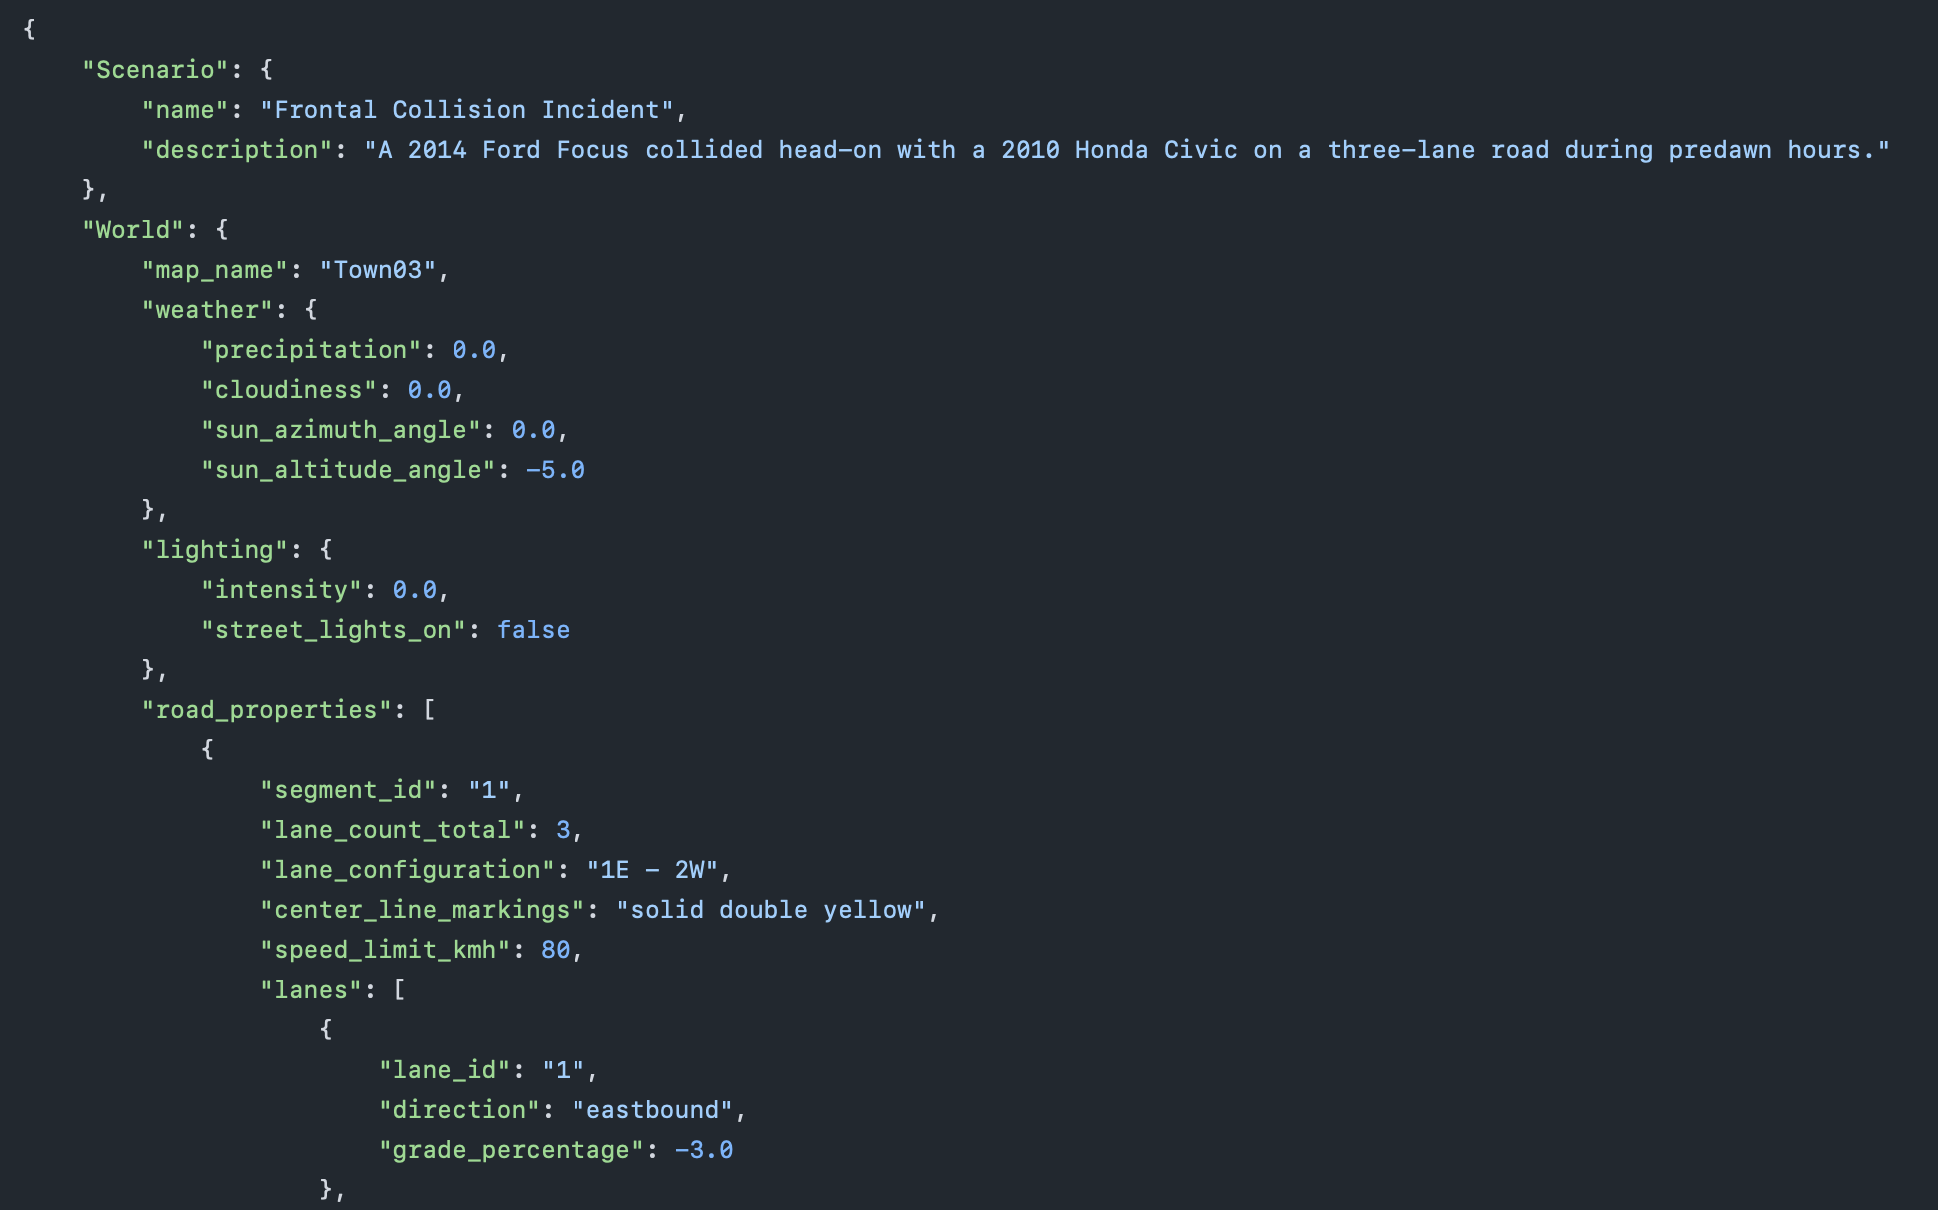
\includegraphics[width=0.8\textwidth]{images/kg-extracted-data-example}
    \caption{ตัวอย่างโครงสร้างข้อมูลที่ได้จากการสกัดรายงานอุบัติเหตุ C00013 โดย Schema-guided LLM}
    \label{fig:ch4_extracted_data}
\end{figure}

\subsection{ขั้นที่ 2: การสร้าง Knowledge Graph (KG Modeling)}\label{subsec:ch4_kg_modeling}

\paragraph{}
ข้อมูลที่มีโครงสร้างจากขั้นตอนที่ 1 จะถูกนำมาสร้างเป็น Knowledge Graph (KG) ซึ่งทำหน้าที่เป็น Semantic Backbone ของข้อมูลอุบัติเหตุทั้งหมด โดยการแปลงข้อมูลแต่ละส่วนให้เป็นโหนด (Nodes) และความสัมพันธ์ (Relationships) ดังกระบวนการใน Function \Call{BuildKnowledgeGraph}{}

\begin{algorithmic}[1]
\Function{BuildKnowledgeGraph}{\textit{graph, data}}
    \Comment{แปลงข้อมูล JSON เป็น Nodes และ Relationships}
    \State Create Nodes for actors, events, environment from \textit{data}
    \State Create Relationships (e.g., :CAUSED\_BY, :OCCURRED\_IN) between nodes
    \State Add nodes and relationships to \textit{graph}
\EndFunction
\end{algorithmic}

\paragraph{}
ผลลัพธ์ที่ได้คือ Knowledge Graph ที่สามารถแสดงความเชื่อมโยงที่ซับซ้อนของปัจจัยต่างๆ ในอุบัติเหตุได้อย่างชัดเจน ดังตัวอย่างในรูปที่~\ref{fig:ch4_kg_model}

\begin{figure}[htbp]
    \centering
    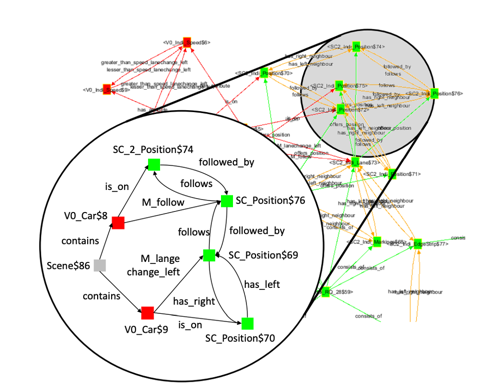
\includegraphics[width=1\textwidth]{images/kg-model-example}
    \caption{ตัวอย่างส่วนหนึ่งของ Knowledge Graph ที่แสดงความสัมพันธ์ของเอนทิตีในอุบัติเหตุ C00013}
    \label{fig:ch4_kg_model}
\end{figure}


\subsection{ขั้นที่ 3: การบูรณาการ ODD และการค้นหา Edge-Case ด้วย Query Rotation}\label{subsec:ch4_odd_integration}

\paragraph{}
ขั้นตอนนี้คือหัวใจสำคัญของกรอบการทำงานซึ่งใช้เทคนิค Query Rotationเพื่อค้นหาสถานการณ์ที่ท้าทายระบบ (Edge-Case) อย่างเป็นระบบ โดยใช้ ODD Modular ซึ่งเป็นกลุ่มของเงื่อนไข ODD ที่ถูกกำหนดไว้ล่วงหน้าเพื่อแทนสถานการณ์อันตรายประเภทต่างๆ (เช่น กลุ่ม "การชนท้าย") จากนั้น อัลกอริทึมจะวนลูปเพื่อสืบค้น (Query) เหตุการณ์ใน Knowledge Graph ทีละ Modular ทำให้มั่นใจได้ว่ามีการค้นหาที่ครอบคลุมในทุกมิติของความเสี่ยง กระบวนการนี้สรุปได้ดัง Function \Call{QueryCasesByModular}{}

\begin{algorithmic}[1]
\Function{QueryCasesByModular}{\textit{graph, modularGroup}}
    \State \textit{InferenceEngine} $\gets$ InitializeEngine(\textit{graph})
    \State \textit{rules} $\gets$ modularGroup.getRules()
    \State \textit{MatchingEvents} $\gets$ \textit{InferenceEngine}.query(\textit{rules})
    \Comment{เช่น ค้นหา Event ที่ตรงตามเงื่อนไขของ Modular ที่กำหนด}
    \State \textbf{return} \textit{MatchingEvents}
\EndFunction
\end{algorithmic}

\paragraph{}
เมื่อระบบทำงานกับ Modular "การฝ่าฝืนสัญญาณจราจร" Inference Engine จะค้นหาเหตุการณ์ทั้งหมดใน KG ที่เข้าข่ายเงื่อนไขนี้ เช่น `Event\_RunRedLight` ในกรณี C00013 และระบุว่าเป็น Edge-Case ที่ตรงกับ Modular ดังกล่าว ดังแสดงในรูปที่~\ref{fig:ch4_kg_inference}

\begin{figure}[htbp]
    \centering
    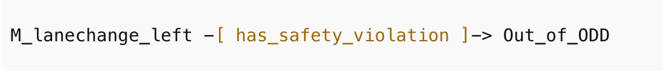
\includegraphics[width=1\textwidth]{images/kg-inference-example}
    \caption{Knowledge Graph หลังจากผ่าน Inference Engine โดยมีการสร้างความสัมพันธ์ใหม่ (เส้นสีแดง) เพื่อระบุว่าเหตุการณ์ฝ่าไฟแดงเป็น Edge-Case ที่ตรงกับ ODD Modular "การฝ่าฝืนสัญญาณจราจร"}
    \label{fig:ch4_kg_inference}
\end{figure}

\subsection{ขั้นที่ 4: การสร้างชุดพารามิเตอร์สำหรับ Scenario Template}\label{subsec:ch4_scenario_generation}

\paragraph{}
ในขั้นตอนสุดท้าย กรอบการทำงานไม่ได้สร้างไฟล์ `.xosc` ออกมาโดยตรง แต่จะดำเนินการในลักษณะที่ยืดหยุ่นกว่า คือการสร้าง ชุดพารามิเตอร์ (Parameter Set) จากข้อมูล Edge-Case ที่ค้นพบในขั้นตอนที่ 3 พารามิเตอร์เหล่านี้คือค่าตัวแปรที่สำคัญของสถานการณ์ เช่น ความเร็วเริ่มต้นของรถ, ตำแหน่ง, ประเภทของยานพาหนะ, สภาพถนน เป็นต้น

\begin{algorithmic}[1]
\Function{GenerateParametersFromEvent}{\textit{eventData}}
    \Comment{Map ข้อมูลจาก KG node ไปเป็นโครงสร้าง Key-Value}
    \State \textit{params} $\gets$ new Dictionary()
    \State \textit{params}["initial\_speed\_v1"] $\gets$ \textit{eventData}.getVehicle(1).speed
    \State \textit{params}["road\_friction"] $\gets$ \textit{eventData}.getEnvironment().surfaceFriction
    \State \textit{params}["maneuver\_actor"] $\gets$ \textit{eventData}.getActor().id
    \State \textbf{return} \textit{params}
\EndFunction
\end{algorithmic}

\paragraph{}
ชุดพารามิเตอร์ที่ได้นี้จะถูกจัดเก็บไว้ และในขั้นตอนการทดสอบจริง ผู้ใช้จะเลือก Scenario Template (เช่น Template สำหรับสถานการณ์ Cut-in, Template สำหรับสถานการณ์ Unsignalized Left-Turn) ซึ่งเป็นไฟล์ `.xosc` ที่มีโครงสร้างทั่วไปและมีช่องว่างสำหรับรับค่าพารามิเตอร์ จากนั้นจึงนำชุดพารามิเตอร์ที่ Framework สร้างขึ้นไปเติมใน Template เพื่อสร้างเป็น Test Case ที่สมบูรณ์และพร้อมใช้งานต่อไป วิธีการนี้ช่วยแยกส่วนระหว่าง "ข้อมูล" (Parameters) และ "ตรรกะของสถานการณ์" (Template) ออกจากกัน ทำให้สามารถสร้าง Test Case ที่หลากหลายได้อย่างมีประสิทธิภาพและนำกลับมาใช้ซ้ำได้ง่าย
\section{ขั้นตอนการประเมินผล: Scenario Completeness Score}\label{sec:ch4_evaluation_method}
\paragraph{}
เพื่อให้สามารถประเมินคุณภาพของสถานการณ์จำลองที่สร้างขึ้นได้อย่างเป็นรูปธรรมและมีมาตรฐาน กรอบการทำงานนี้ได้กำหนดวิธีการประเมินเชิงปริมาณที่เรียกว่า \textbf{Scenario Completeness Score} (หรือ R-score) ขึ้นมา โดยมีวัตถุประสงค์เพื่อวัดคุณภาพเชิงฟังก์ชัน (Functional Quality) ของ Knowledge Graph ที่ได้จากระบบ เปรียบเทียบกับกราฟต้นฉบับ (Ground Truth) ที่สร้างขึ้นจากรายงานอุบัติเหตุจริง

\paragraph{}
หัวใจสำคัญของการประเมินคือการให้น้ำหนัก (Weighting) กับความสัมพันธ์ (Edges/Relationships) แต่ละประเภทตามความสำคัญที่มีต่อความสมจริงของสถานการณ์ (Scenario Fidelity) โดยคำนวณจากสูตรดังสมการที่~\ref{eq:completeness_score}

\begin{equation}
    \text{Score}_{\text{Weighted}} = \frac{\sum_{\text{Common Edges}} W_i}{\sum_{\text{All Edges in Both Graphs}} W_i}
    \label{eq:completeness_score}
\end{equation}

\paragraph{}
โดยที่:
\begin{itemize}
    \item \textbf{ตัวเศษ ($\sum_{\text{Common Edges}} W_i$):} คือผลรวมของค่าน้ำหนัก ($W_i$) ของความสัมพันธ์ทั้งหมดที่ปรากฏ \textbf{ร่วมกัน} ทั้งในกราฟต้นฉบับและกราฟที่ระบบสร้างขึ้น ซึ่งสะท้อนถึงองค์ประกอบของสถานการณ์ที่ระบบสามารถสร้างได้อย่างถูกต้อง
    \item \textbf{ตัวส่วน ($\sum_{\text{All Edges in Both Graphs}} W_i$):} คือผลรวมของค่าน้ำหนัก ($W_i$) ของความสัมพันธ์ทั้งหมดที่ไม่ซ้ำกันที่ปรากฏในกราฟใดกราฟหนึ่งหรือทั้งสองกราฟรวมกัน ซึ่งสะท้อนถึงข้อมูลที่เป็นไปได้ทั้งหมดของสถานการณ์
\end{itemize}

\paragraph{}
ค่าน้ำหนัก ($W_i$) ถูกกำหนดขึ้นโดยแบ่งตามประเภทและความสำคัญของความสัมพันธ์ ดังแสดงในตารางที่~\ref{tab:relationship_weights}

\begin{table}[htbp]
    \centering
    \caption{ค่าน้ำหนักของความสัมพันธ์ประเภทต่างๆ ตามความสำคัญต่อความสมจริงของสถานการณ์}
    \label{tab:relationship_weights}
    \begin{tabular}{|l|c|p{7cm}|}
        \hline
        \rowcolor{gray!20} \textbf{Relationship Type} & \textbf{Weight ($W_i$)} & \textbf{Importance to Scenario Fidelity} \\
        \hline
        Temporal/Causal & 3 & จำเป็นอย่างยิ่งต่อการกำหนดลำดับเหตุการณ์และความเป็นเหตุเป็นผลของอุบัติเหตุ \\
        (เช่น followed\_by, M\_follow) & & \\
        \hline
        Positional/Topological & 2 & จำเป็นต่อการกำหนดบริบทเชิงพื้นที่และขอบเขตของ ODD ที่แม่นยำ \\
        (เช่น is\_on, adjacent\_left) & & \\
        \hline
        Proximity/Trigger & 1 & จำเป็นต่อการกำหนดเงื่อนไขเริ่มต้น (Start Trigger) ของเหตุการณ์วิกฤต \\
        (เช่น near\_coll, very\_near) & & \\
        \hline
    \end{tabular}
\end{table}

\paragraph{}
ค่าคะแนนที่ได้จะมีค่าอยู่ระหว่าง 0 ถึง 1 โดยคะแนนที่เข้าใกล้ 1 หมายถึงกราฟที่ระบบสร้างขึ้นมีความสมบูรณ์และความสมจริงสูง สามารถจำลององค์ประกอบเชิงฟังก์ชันที่สำคัญของอุบัติเหตุต้นฉบับได้อย่างครบถ้วน

\section{ข้อจำกัดของการศึกษา}\label{sec:ch4_limitations}
\paragraph{}

การวิจัยนี้มุ่งเน้นการพัฒนากรอบการทำงานที่เป็นแนวคิดใหม่ในการสร้างชุดทดสอบ แต่ก็มีข้อจำกัดหลายประการที่ต้องนำมาพิจารณา ซึ่งส่วนใหญ่เกี่ยวข้องกับคุณภาพของข้อมูลนำเข้า ความจำกัดของเทคโนโลยีที่ใช้ และขอบเขตการดำเนินงานที่ถูกกำหนดไว้ล่วงหน้า ดังนี้:

\subsection{ข้อจำกัดด้านข้อมูลและเทคโนโลยี}

\begin{enumerate}
    \item \textbf{การพึ่งพาข้อมูลอุบัติเหตุในอดีต:} การศึกษานี้ขึ้นอยู่กับรายงานอุบัติเหตุจริงจากฐานข้อมูลสาธารณะ เช่น CIREN และ GIDAS ซึ่งเป็นข้อมูลในอดีตและมีลักษณะที่ไม่สมบูรณ์ รวมถึงมีความเป็นอัตวิสัย (Subjectivity) ในการบันทึกของผู้รายงาน ข้อจำกัดนี้ส่งผลโดยตรงต่อคุณภาพและความแม่นยำของ Knowledge Graph ที่ถูกสร้างขึ้น
    \item \textbf{ความท้าทายด้านความน่าเชื่อถือของ LLM:} แม้จะมีการใช้ Schema-guided LLM เพื่อสกัดข้อมูล แต่โมเดลภาษายังคงมีแนวโน้มที่จะสร้างข้อมูลที่ผิดพลาด (Hallucination) หรือความสัมพันธ์เชิงเหตุผลที่ไม่ถูกต้อง โดยเฉพาะในสถานการณ์อุบัติเหตุที่มีความซับซ้อน ซึ่งทำให้ต้องอาศัยการตรวจสอบและปรับแก้จากผู้เชี่ยวชาญเพิ่มเติม
    \item \textbf{ข้อจำกัดในการสรุปผล ODD และการออกแบบ Modular:} Operational Design Domain (ODD) ที่ใช้ในการวิจัยนี้อ้างอิงตามมาตรฐานของ JAMA เป็นหลัก ดังนั้นผลลัพธ์ที่ได้จึงอาจไม่สามารถนำไปประยุกต์ใช้โดยตรงกับระบบ ADS ที่มีนิยาม ODD แตกต่างกัน นอกจากนี้ การจัดกลุ่มเงื่อนไขเป็น ODD Modular เพื่อใช้ในเทคนิค Query Rotation อาจมีความเป็นอัตวิสัยในการออกแบบ ซึ่งอาจส่งผลต่อประเภทและลำดับความสำคัญของ Edge-Case ที่ถูกค้นพบ
    \item \textbf{ปัญหาด้านการประมวลผลของ Knowledge Graph:} เมื่อ Knowledge Graph เติบโตขึ้นตามจำนวนรายงานอุบัติเหตุที่เพิ่มขึ้น ประสิทธิภาพในการประมวลผลของ Inference Engine เพื่อสืบค้นและประเมินกฎ ODD ในแต่ละ Modular จะลดลง ซึ่งอาจเป็นข้อจำกัดในการนำกรอบการทำงานนี้ไปใช้งานในระดับอุตสาหกรรมขนาดใหญ่ที่ต้องการความรวดเร็ว
\end{enumerate}

\subsection{ข้อจำกัดด้านขอบเขตการดำเนินงาน}

\begin{enumerate}
    \item \textbf{ผลลัพธ์สิ้นสุดที่การสร้างพารามิเตอร์:} ขอบเขตของโครงการสิ้นสุดที่การสร้าง ชุดพารามิเตอร์ (Parameter Set) สำหรับนำไปใช้กับ Scenario Template และไม่ได้รวมถึงการดำเนินการจำลองสถานการณ์ (Simulation) หรือการทดสอบภาคสนามจริง ดังนั้น การประเมินผลกระทบที่แท้จริงของชุดทดสอบต่อประสิทธิภาพของระบบ ADS จึงอยู่นอกเหนือขอบเขตของการศึกษานี้
    \item \textbf{การพึ่งพาคุณภาพของ Scenario Template:} ประสิทธิภาพของ Test Case สุดท้ายที่สร้างขึ้น ไม่ได้ขึ้นอยู่กับคุณภาพของพารามิเตอร์ที่กรอบการทำงานนี้สร้างขึ้นเท่านั้น แต่ยังขึ้นอยู่กับคุณภาพ ความถูกต้อง และความครอบคลุมของ Scenario Template เช่น ไฟล์ `.xosc` ที่มีอยู่ก่อนแล้ว หาก Template มีข้อบกพร่องหรือไม่ครอบคลุมสถานการณ์ที่หลากหลาย ก็จะจำกัดประโยชน์ของพารามิเตอร์ที่สร้างขึ้น
    \item \textbf{การละเลยปัจจัยมนุษย์ในระดับละเอียด:} Scenario ที่สร้างขึ้นเน้นการจับภาพเหตุการณ์ทางกายภาพและสภาพแวดล้อมเป็นหลัก แม้จะมีการเก็บข้อมูลพฤติกรรม แต่การวิเคราะห์และจำลองปัจจัยด้านมนุษย์ (Human Factors) เช่น ความผิดพลาดทางสติปัญญา หรือการตอบสนองทางอารมณ์ของผู้ขับขี่อย่างละเอียด ยังคงเป็นสิ่งที่ซับซ้อนและไม่ได้เป็นจุดเน้นหลักของกรอบการทำงานนี้
\end{enumerate}
\chapter{ผลการศึกษา}

\section{ผลการดำเนินงานตามวัตถุประสงค์}

แสดงวัตถุประสงค์แต่ละข้อและผลที่ได้ว่าสอดคล้องกันหรือไม่

\section{ตัวอย่างผลลัพธ์}

แสดงผลลัพธ์ที่ได้จากระบบ เช่น หน้าจอโปรแกรม ตาราง หรือกราฟ

\section{การเปรียบเทียบก่อนและหลังการพัฒนา}

เปรียบเทียบประสิทธิภาพหรือกระบวนการก่อนและหลังมีระบบ

\section{การประเมินผล}

รายงานผลการประเมินจากผู้ใช้หรือเกณฑ์ทางเทคนิคที่กำหนด
\chapter{สรุปผลการศึกษาและวิจารณ์ผลการศึกษา}

\section{สรุปผลการดำเนินงาน}

สรุปผลสำเร็จของโครงการอย่างกระชับและครอบคลุม

\section{ข้อสังเกตและข้อวิจารณ์}

สะท้อนถึงประเด็นที่น่าสนใจหรือจุดที่ยังควรปรับปรุง

\section{ข้อเสนอแนะในการพัฒนาต่อไป}

เสนอแนวทางหรือฟีเจอร์เพิ่มเติมที่ควรมีในอนาคต

\section{ประสบการณ์จากการเข้าร่วมโครงการสหกิจศึกษา}

ถ่ายทอดสิ่งที่ผู้เขียนได้เรียนรู้จากการทำงานจริงในองค์กร

\bibliographystyle{ieeetr}
\bibliography{references}

\end{document}